% !TeX TXS-program:compile = txs:///arara
% arara: lualatex: {shell: no, synctex: yes, interaction: batchmode}
% arara: pythontex: {rerun: modified} if exists('pytxcode') && found('pytxcode', 'PYTHONTEX#py')
% arara: lualatex: {shell: no, synctex: yes, interaction: batchmode} if exists('pytxcode') && found('pytxcode', 'PYTHONTEX#py')
% arara: lualatex: {shell: no, synctex: yes, interaction: batchmode} if found('log', '(undefined references|Please rerun|Rerun to get)')

\documentclass[a4paper,11pt]{article}
\usepackage[revgoku]{cp-base}
\graphicspath{{./graphics/}}
%variables
\donnees[classe={1\up{ère} 2M2},matiere={[SPÉ.MATHS]},mois=Mai,annee=2022,typedoc=CHAP,numdoc=11]

%formatage
\author{Pierquet}
\title{\nomfichier}
\hypersetup{pdfauthor={Pierquet},pdftitle={\nomfichier},allbordercolors=white,pdfborder=0 0 0,pdfstartview=FitH}
%divers
\lhead{\entete{\matiere}}
\chead{\entete{\lycee}}
\rhead{\entete{\classe{} - \mois{} \annee}}
\lfoot{\pied{\matiere}}
\cfoot{\logolycee{}}
\rfoot{\pied{\numeropagetot}}

\begin{document}

\pagestyle{fancy}

\part{CH11 - Applications de la dérivation - Exercices (Correction)}

\medskip

\exonum{0}

\begin{enumerate}
	\item On utilise le théorème fondamental pour passer du tds de $g'(x)$ au tdv de $g$ :
	\begin{center}
		\begin{tikzpicture}
			\tkzTabInit{$x$/0.6,$g'(x)$/0.6,$g$/1.2}{$0$,$3$,$6$,$+\infty$}
			\tkzTabLine{,-,z,+,z,-,}
			\tkzTabVar{+/$g(0)$,-/$-1$,+/$2$,-/}
		\end{tikzpicture}
	\end{center}
	\item On peut proposer la courbe {\red $\mathscr{C}_g$} suivante (on a choisi $g(0)=4$) :
	\begin{center}
		\tunits{0.75}{0.75}
		\tdefgrille{-1}{12}{1}{1}{-5}{5}{1}{1}
		\begin{tikzpicture}[x=\xunit cm,y=\yunit cm]
			%grilles & axes
			\tgrilles[line width=0.3pt,lightgray!50] ;
			\tgrillep[line width=0.6pt,lightgray!50] ;
			\axestikz* ;
			\axextikz[]{-1,0,...,11} ;
			\axeytikz[]{-5,-4,...,4} ;
			\clip (\xmin,\ymin) rectangle (\xmax,\ymax) ; %on restreint les fonctions à la fenêtre
			%splines
			\def\LISTE{0/4/-3§3/-1/0§6/2/0§12/-10/-8}
			\splinetikz[liste=\LISTE,couleur=red,coeffs=2§3§2]
			%divers
			\draw[red] (10.75,-3) node {\large $\mathscr{C}_g$} ;
			\foreach \x/\y in {3/-1,6/2}{%
				\filldraw[darkgray] (\x,\y) circle[radius=2.5pt] ;
				\draw[darkgray,very thick,<->,>=stealth] ({\x-1.5},\y) -- ({\x+1.5},\y) ;
				}
		\end{tikzpicture}
	\end{center}
\end{enumerate}

\medskip

\exonum{1}


\begin{enumerate}
	\item Le maximum local de $k$ sur $\intervFF{-8}{-4}$ est $1$, atteint en $x=-5$.
	\item Le minimum local de $k$ sur $\intervFF{-8}{0}$ est $-1$, atteint en $x=-4$.
	\item Le maximum de $k$ sur $\intervFF{-8}{6}$ est $7$, atteint en $x=6$.
	\item Le minimum de $k$ au voisinage de $3$ est $0$, atteint en $x=3$.
\end{enumerate}

\exonum{1}

\begin{enumerate}
	\item La fonction $f$ est dérivable sur $\R$ (polynôme), et $f'(x)=-3x^2+2x+1$.
	\item $f'(x)$ est un trinôme :
	\begin{itemize}
		\item $\Delta=16$ et les deux racines sont $x_1=1$ et $x_2=-\tfrac13$ ;
		\item $a=-3$ donc le signe est $\ominus\oplus\ominus$.
	\end{itemize}
	\begin{center}
		\begin{tikzpicture}
			\tkzTabInit[]{$x$/0.8,$f'(x)$/0.8,$f$/1.6}{$-\infty$,$-\tfrac13$,$1$,$+\infty$}
			\tkzTabLine{,-,z,+,z,-,}
			\tkzTabVar{+/,-/$\tfrac{49}{27}$,+/$3$,-/}
			\draw ($(T20)!0.5!(T23)$) node[right=3pt] {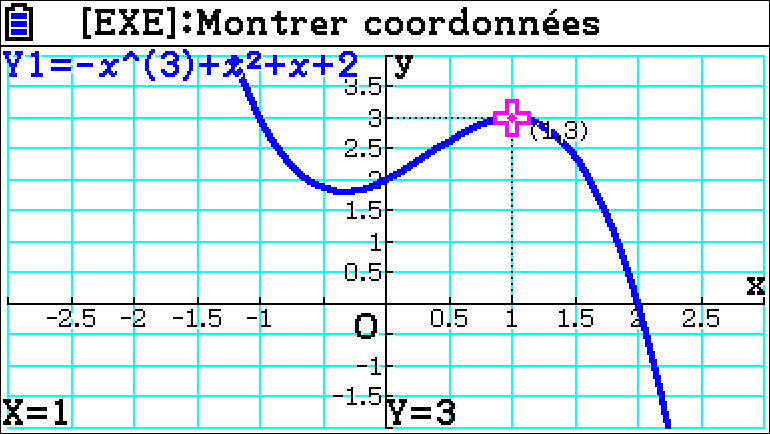
\includegraphics[width=3.85cm]{td09_corr_exo3}} ; 
		\end{tikzpicture}
		
		Avec $f(1)=3$ et $f\left(-\tfrac13\right)=\tfrac{49}{27}$.
	\end{center}
\end{enumerate}

\medskip

\exonum{2}

\begin{enumerate}
	\item Le dénominateur de $h(x)$ ne s'annule pas sur $\R$ : c'est un trinôme avec $\Delta=-4<0$, donc $\mathcallig{D}_h=\R$.
	
	De plus, comme fraction rationnelle définie sur $\R$, $h$ est dérivable sur $\R$ et, par quotient :
	
	$h'(x)=\dfrac{(-2x+8) \times (x^2-4x+5)-(2x-4) \times (-x^2+8x+13)}{\big( x^2-4x+5\big)^2}$
	
	$\phantom{h'(x)}=\dfrac{-2x^3+8x^2-10x+8x^2-32x+40-(-2x^3+16x^2+26x+4x^2-32x-52)}{\big( x^2-4x+5\big)^2}=\dfrac{-4x^2+16x-12}{\big( x^2-4x+5\big)^2}$ sur $\R$.
	\item On étudie le signe de $h'(x)$, qui s'exprime comme un quotient :
	\begin{itemize}
		\item $-4x^2+16x-12$ est un trinôme : $\Delta=64$ et les deux racines sont $x_1=1$ et $x_2=3$ avec $a=-4<0$ ;
		\item $\big( x^2-4x+5\big)^2$ est le carré d'un trinôme ne s'annulant jamais, il est donc toujours strictement positif.
	\end{itemize}
	\begin{center}
		\begin{tikzpicture}
			\tkzTabInit[lgt=3.15]{$x$/0.8,$-4x^2+16x-12$/0.8,$\big( x^2-4x+5\big)^2$/0.8,$h'(x)$/0.8,$h$/1.6}{$-\infty$,$1$,$3$,$+\infty$}
			\tkzTabLine{,-,z,+,z,-,}
			\tkzTabLine{,+,t,+,t,+,}
			\tkzTabLine{,-,z,+,z,-,}
			\tkzTabVar{+/,-/$-3$,+/$1$,-/}
			\draw ($(T20)!0.5!(T25)$) node[right=3pt] {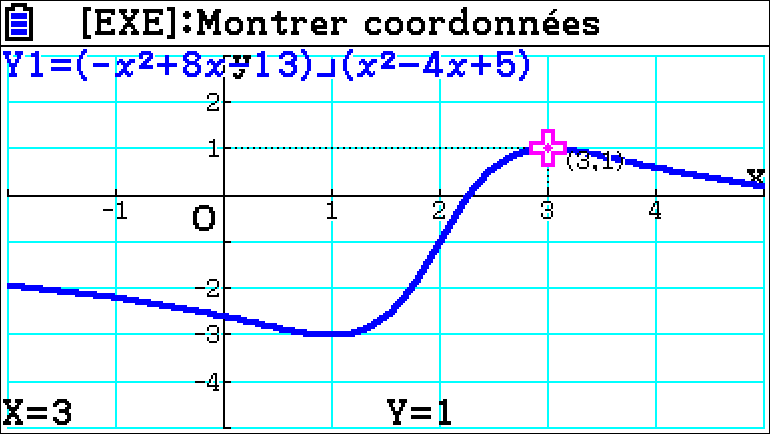
\includegraphics[width=3.85cm]{td09_corr_exo4}} ; 
		\end{tikzpicture}
		
		Avec $h(1)=-3$ et $h(3)=1$.
	\end{center}
\end{enumerate}

\medskip

\exonum{2}

\begin{enumerate}
	\item La fonction $f$ est dérivable sur $\intervFF{1}{6}$ (somme de fonctions dérivables).
	
	Et on a $f'(x)=2-0+8 \times \dfrac{-1}{x^2}=\dfrac{2x^2-8}{x^2}$ pour tout réel $x \in \intervFF{1}{6}$.
	\item On étudie le signe de $f'(x)$, qui s'exprime comme un quotient :
	\begin{itemize}
		\item $2x^2-8$ est un trinôme : $\Delta=64$ et les deux racines sont $x_1=2$ et $x_2=-2$ avec $a=2>0$ ;
		\item $x^2$ est toujours strictement positif sur $\intervFF{1}{6}$.
	\end{itemize}
	\begin{center}
		\begin{tikzpicture}
			\tkzTabSetup[fromcolor=red,fromstyle=densely dotted]
			\tkzTabInit[]{$x$/0.8,$2x^2-8$/0.8,$x^2$/0.8,$f'(x)$/0.8,$f$/1.6}{$1$,$2$,$6$}
			\tkzTabLine{,-,z,+,}
			\tkzTabLine{,+,t,+,}
			\tkzTabLine{,-,z,+,}
			\tkzTabVar{+/$0$,-/$-2$,+/$\tfrac{10}{3}$}
			\tkzTabVal[draw]{2}{3}{0.35}{\small \red $4$}{\small \red $0$}
			\draw ($(T20)!0.5!(T25)$) node[right=3pt] {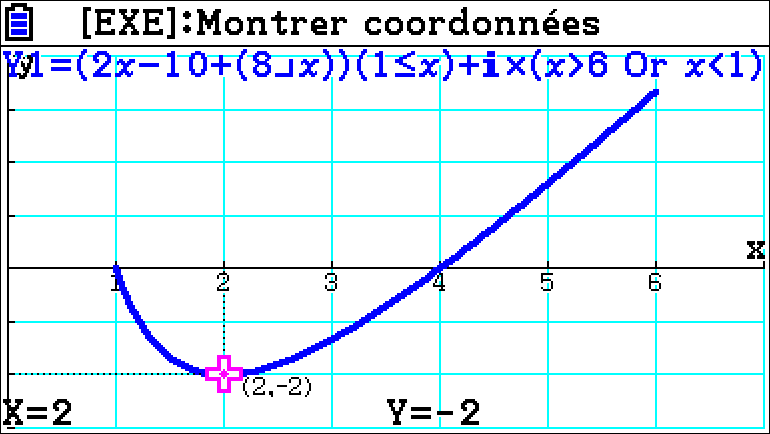
\includegraphics[width=3.85cm]{td09_corr_exo5}} ; 
		\end{tikzpicture}
		
		Avec $f(1)=0$ ; $f(2)=-2$ et $f(6)=\tfrac{10}{3}$.
	\end{center}
	\item On peut en déduire que $f$ admet un minimum sur $I$, qui vaut $-2$ et qui est atteint en $x=2$.
	\item Les différentes données du tdv de $f$ permettent de déduire le tds de $f(x)$ (on \og descend les $0$ \fg\ldots) :
	\begin{center}
		\begin{tikzpicture}
			\tkzTabInit[]{$x$/0.8,$f(x)$/0.8}{$1$,$4$,$6$}
			\tkzTabLine{z,-,z,+,}
		\end{tikzpicture}
	\end{center}
	\item On arrive à \og placer \fg{} {\blue $-1$} sur les 2 flèches du tdv de $f$, c'est donc que l'équation $f(x)=1$ admet {\blue 2} solutions.
	\begin{center}
		\begin{tikzpicture}
			\tkzTabSetup[fromcolor=blue,fromstyle=densely dotted]
			\tkzTabInit[]{$x$/0.8,$f$/1.6}{$1$,$2$,$6$}
			\tkzTabVar{+/$0$,-/$-2$,+/$\tfrac{10}{3}$}
			\tkzTabVal[draw]{1}{2}{0.6}{\small \blue $\alpha$}{\small \blue $-1$}
			\tkzTabVal[draw]{2}{3}{0.4}{\small \blue $\beta$}{\small \blue $-1$}
		\end{tikzpicture}
	\end{center}
\end{enumerate} 

\medskip

\exonum{2}

\begin{enumerate}
	\item On lit graphiquement le tdv de $f$ pour en déduire le tds de $f'(x)$ (grâce au thm fondamental) :
	\begin{center}
		\begin{tikzpicture}
			\tkzTabInit[]{$x$/0.6,$f$/1.3,$f'(x)$/0.6}{$-\infty$,$-1$,$0$,$2$,$+\infty$}
			\tkzTabVar{-/,+/$a$,-/$b$,+/$3$,-/}
			\tkzTabLine{,+,z,-,z,+,z,-,}
		\end{tikzpicture}
	\end{center}
	\item Parmi les 3 courbes proposées, la seule compatible (au niveau du signe $\oplus\ominus\oplus\ominus$) est \textcolor{ForestGreen}{$\mathscr{C}_3$}.
\end{enumerate}

\medskip

\exonum{3}

%Soit $f$ la fonction définie et (deux fois) dérivable sur $\R$ par $f'(x)=3x^4-4x^3+6x^2-12x+12$.

\begin{enumerate}
	\item $f$ est dérivable sur $\R$ (polynôme) et $f'(x)=3 \times 4x^3-4 \times 3x^2+6 \times 2x - 12=12x^3-12x^2+12x-12$ pour tout $x$.
	
	$f'$ est dérivable sur $\R$ (polynôme) et $f''(x)=12 \times 3x^2-12 \times 2x + 12=36x^2-24x+12$ pour tout $x$.
	\item
	\begin{enumerate}
		\item $f''(x)$ est un trinôme : $\Delta = \num{-1152}$, pas de racine réelle, et $a=36>0$.
		\begin{center}
			\begin{tikzpicture}
				\tkzTabInit[espcl=5]{$x$/0.6,$f''(x)$/0.6}{$-\infty$,$+\infty$}
				\tkzTabLine{,+,}
			\end{tikzpicture}
		\end{center}
		\item On en déduit (thm fondamental) de tdv de $f'$ :
		\begin{center}
			\begin{tikzpicture}
				\tkzTabSetup[fromcolor=red,fromstyle=densely dotted]
				\tkzTabInit[espcl=5]{$x$/0.6,$f''(x)$/0.6,$f'$/1.3}{$-\infty$,$+\infty$}
				\tkzTabLine{,+,}
				\tkzTabVar{-/,+/}
				\tkzTabVal[draw]{1}{2}{0.62}{\red $1$}{\red $0$}
			\end{tikzpicture}
		\end{center}
	\end{enumerate}
	\item 
	\begin{enumerate}
		\item On a $f'(1)=0$ ce qui permet de déduire le signe de $f'(x)$ sur $\R$ (\og on descend les $0$ \fg\ldots) :
		\begin{center}
			\begin{tikzpicture}
				\tkzTabInit[]{$x$/0.68,$f'(x)$/0.6}{$-\infty$,$1$,$+\infty$}
				\tkzTabLine{,-,z,+,}
			\end{tikzpicture}
		\end{center}
		\item On peut finalement dresser finalement le tableau de variations de $f$ sur $\R$ (thm fondamental) :
		\begin{center}
			\begin{tikzpicture}
				\tkzTabInit[]{$x$/0.8,$f'(x)$/0.6,$f$/1.3}{$-\infty$,$1$,$+\infty$}
				\tkzTabLine{,-,z,+,}
				\tkzTabVar{+/,-/$5$,+/}
				\draw ($(T20)!0.5!(T23)$) node[right=3pt] {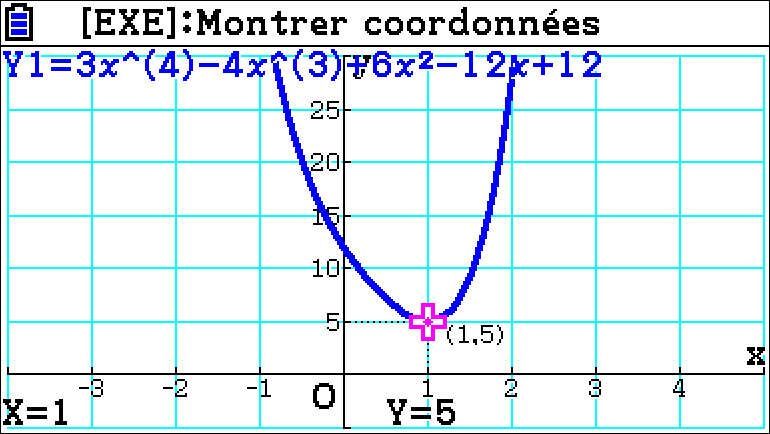
\includegraphics[width=3.85cm]{td09_corr_exo7}} ;
			\end{tikzpicture}
		\end{center}
	\end{enumerate}
\end{enumerate}

\end{document}